\documentclass[11pt,twocolumn,twoside]{IEEEtran}
\usepackage{amsmath}
\usepackage[pdftex]{epsfig}
\usepackage{amsfonts}
\usepackage{amssymb}
\usepackage{fancyhdr}
\usepackage{url}
\include{graphicsx}

\pagestyle{fancy}
%\renewcommand{\headrulewidth}{0pt}
\renewcommand{\footrulewidth}{0pt}
\rhead{
\includegraphics[height=0.6in]{cilogo.png}}
\fancyhead[LO]{\sc sci-wms\ldots} % shorter form of title to fit in space
\fancyhead[LE]{\sc Mayer, McKenna, Foster, Knee} % author list or et al., to fit in space
\chead{}
\cfoot{}

\newcommand{\comt}{COMT}
\newcommand{\ioos}{IOOS}
\newcommand{\sura}{SURA}
\newcommand{\ogc}{OGC}
\newcommand{\wms}{WMS}
\newcommand{\csw}{CSW}
\newcommand{\ugrid}{u-grid}
\newcommand{\cgrid}{c-grid}
\newcommand{\ncml}{NcML}
\newcommand{\noaa}{NOAA}
\newcommand{\ngdc}{NGDC}
\newcommand{\opendap}{OPeNDAP}
\newcommand{\netcdf}{NetCDF}
\newcommand{\sciwms}{SCI-WMS}
\newcommand{\Sciwms}{SCI-WMS}
\newcommand{\adcirc}{ADCIRC}
\newcommand{\fvcom}{FVCOM}
\newcommand{\selfe}{SELFE}
\newcommand{\slosh}{SLOSH}
\newcommand{\mdl}{MDL}
\newcommand{\und}{UND}
\newcommand{\usf}{USF}
\newcommand{\vims}{VIMS}
\newcommand{\umass}{UMASS}
\newcommand{\dal}{DAL}
\newcommand{\tamu}{TAMU}
\newcommand{\http}{HTTP}


\begin{document}
\title{\vspace{0.2in}\sc sci-wms:Python based Web Mapping Service for Visualizing Geospatial data}

%% \author{Brandon A. Mayer$^{1,2}$, Brian McKenna$^{2}$, Dave A. Foster$^{2}$, Kelly Knee$^{2}$\thanks{{Brown University School Of Engineering$^{1}$, RPS ASA, South Kingston RI$^{2}$, Brandon\_Mayer@brown.edu,~BMcKenna@asascience.com,~DFoster@asascience.com,~KKnee@asascience.com}}}

\author{Brandon A. Mayer$^{1,2}$, Brian McKenna$^{2}$, Dave A. Foster$^{2}$, Kelly Knee$^{2}$\thanks{Brown University$^{1}$, RPS ASA, South Kingston RI$^{2}$}\thanks{\{BMayer,BMcKenna,DFoster,KKnee\}@asascience.com}}

\maketitle
\thispagestyle{fancy}

\begin{abstract}
\sciwms{} is an open-source python implementation of an \ogc{}
\wms{}~\cite{wms14} service for qualitatively assessing
society-critical oceanagraphic applications including: forecasting,
risk assessment, model comparison and algorithmic/parameter
selection. The modular cross-platform implementation of \sciwms{}
allows the service to keep pace with the rapid developments in the
geospatial data science community and to produce visualizations for
numerous types of model outputs with transparent support for both
structured and unstructured geo-referenced topologies. This abstract
outlines the implementation and technology stack for visualizing
geospatial Climatological and Forecasting (CF) data using
\sciwms{}\footnote{https://github.com/asascience-open/sci-wms} and
details the deployment of \sciwms{} for visualizing model data and
simulations within the scope of the U.S. \ioos{} Coastal and Ocean
Modeling Testbed project~\cite{luettich13}.
\end{abstract}

\section{Motivation}
The U.S. Integrated Ocean Observing System (\ioos{}) Coastal and Ocean
Modeling Testbed (\comt{}) was formed to unify otherwise disparate
entities in government, academia and industry to leverage the
proliferation of oceanagraphic data and modeling techniques to combat
natural and man-made coastal stressors by accelerating the turnaround
from research and development to operational application of
society-critical applications including: forecasting, model
comparison, model skill assessment, and algorithmic/parameterization
improvements~\cite{luettich13}. Key to the U.S. \ioos{} \comt{}
mission is an extensible and universally available tool for quickly
visualizing and assessing a diverse set of coastal modeling
data. \sciwms{} is a general \ogc{} \wms{} solution for serving
rasterized visualizations of geospatial data which has been deployed
for the \comt{} project to provide visualizations of a wide range of
scientific data.

\section{\sciwms{}}
\Sciwms{} is an open-source implementation of the Open Geospatial
Consortium's (\ogc{}) Web Map Service (\wms{}) standard which
specifies an HTTP interface for generating rasterized visualizations
of geospatial data~\cite{wms14}. \sciwms{} is implemented in Python
using the Django\footnote{\url{https://www.djangoproject.com/}} web
framework and standard cross-platform numerical software, NumPy and
Matplotlib~\cite{numpy11, hunter07} for generating visual
content. Additionally, the open-source python implementation provides
a cross-platform \wms{} solution which can leverage the suite of tools
developed by the geospatial data analysis community such as
pyugrid\footnote{https://github.com/pyugrid/pyugrid} to maintain pace
with the latest geospatial software and standards developments such as
unstructured grid support and CF-UGrid
Compliance\footnote{https://github.com/ugrid-conventions/ugrid-conventions/blob/v0.9.0/ugrid-conventions.md}.

Vital to the efficiency of \sciwms{} is the abstraction
of an oceanagraphic dataset into two entities: a topology, defined as
a geo-referenced spatial structure and numerical model output as
visualized in figure~\ref{fig:sciwms_topology_endpoints}. \Sciwms{}
creates a local topology cache for efficiently computing spatial
neighborhoods with respect to topology structure.  For storage
efficiency, model output is not replicated locally but referenced via
OGC compliant web-services. Because geospatial \wms{} requests are
commonly restricted to a subset of the Earth's surface, \sciwms{} uses
the local topology to compute the subset of model data needed to
fulfill each request prior to accessing the external
data. Furthermore, by classifying topologies as either regular or
unstructured, efficient algorithms and data structures are exploited
to optimize the computation of relevant model data subsets.

\begin{figure}[ht!]
  \centering
  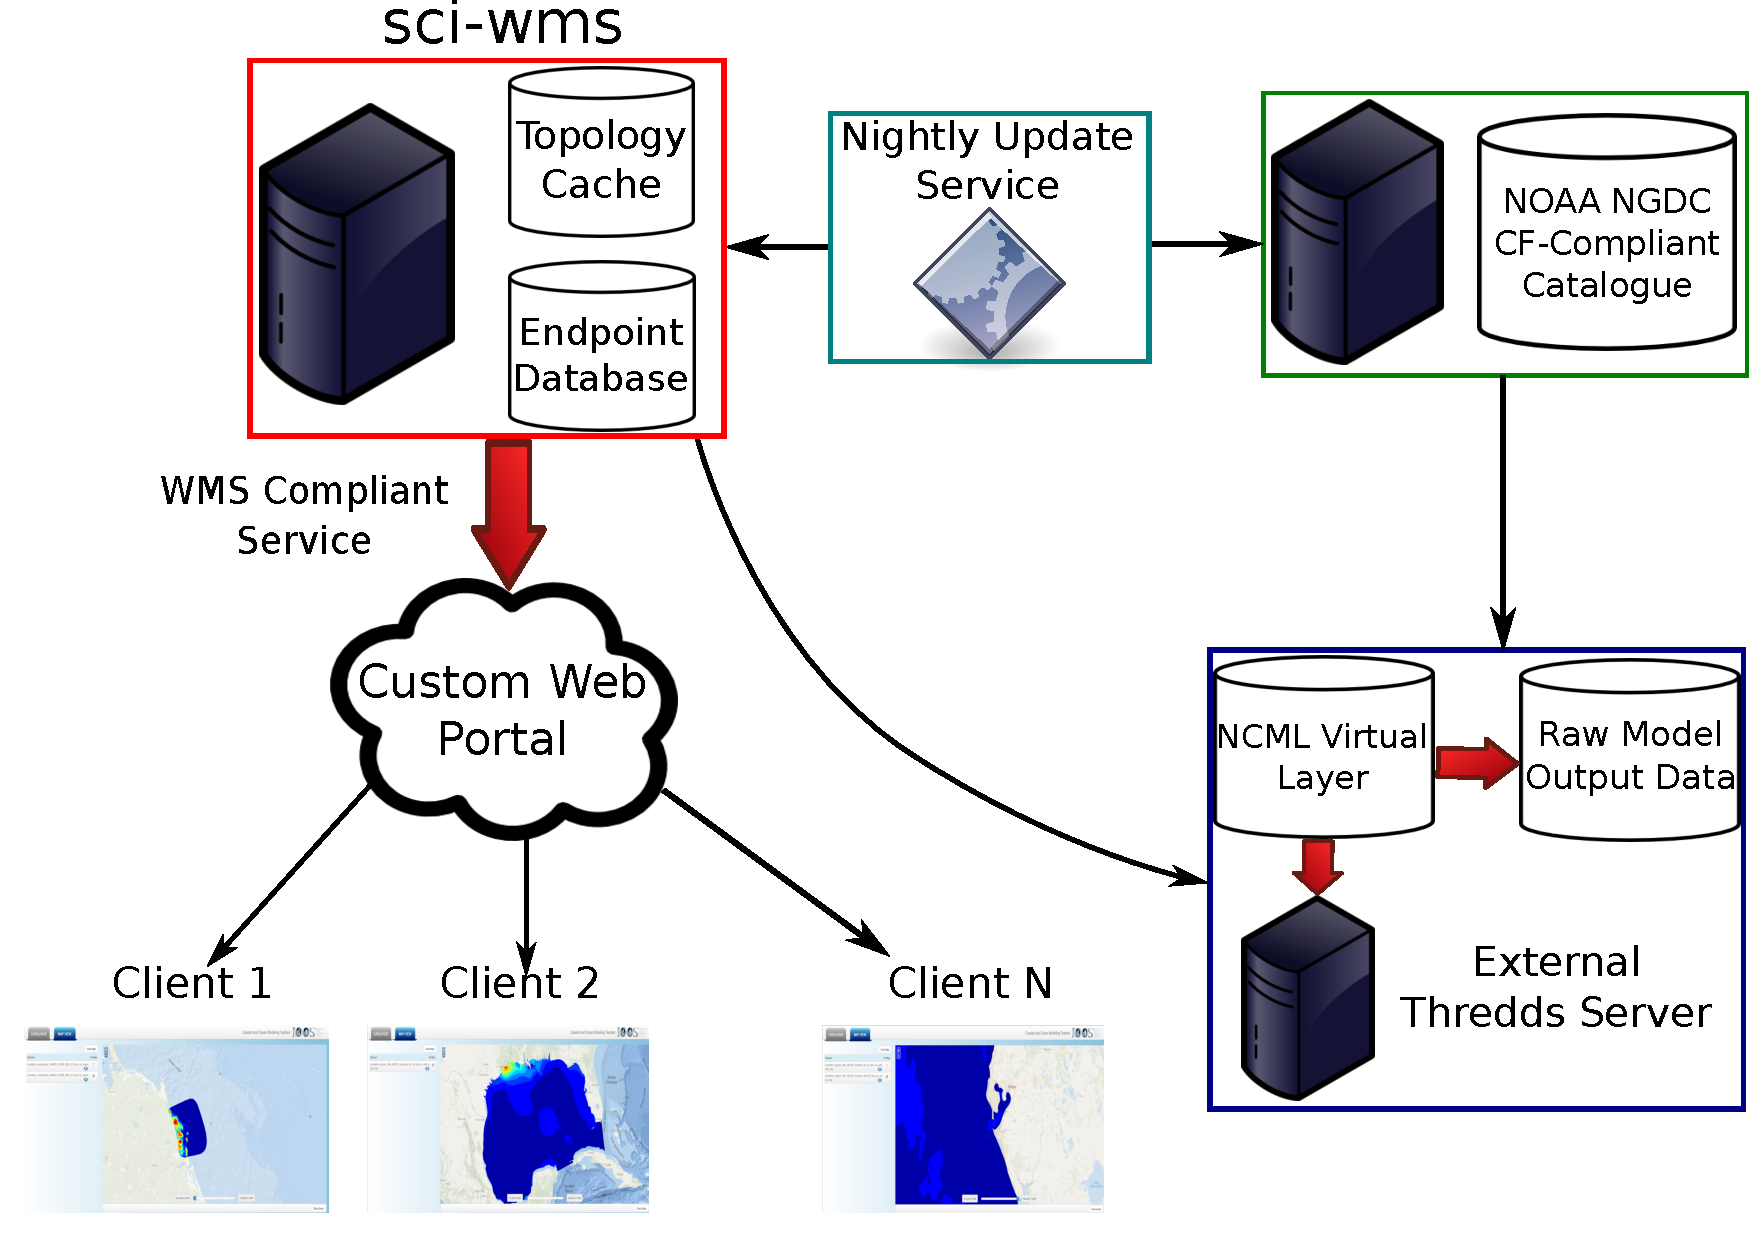
\includegraphics[width=0.7\columnwidth]{./figs/overview.pdf}
  \caption{Overview of the \sciwms{} deployment for the U.S. \ioos{}
    \comt{} project. \Sciwms{} updates its topology and endpoint
    database via a nightly service which queries CF-Compliant datasets
    cataloged by \ngdc{}. Model data is hosted on an external web
    server through an \ncml{} facade accessible to \sciwms{} through
    \opendap{} as a single \netcdf{} data structure. \Sciwms{} then
    responds to http requests made simultaneously by multiple clients
    interfacing through a custom built web-portal.}
  \label{fig:overview1}
\end{figure}

\begin{figure}[ht!]
  \centering
  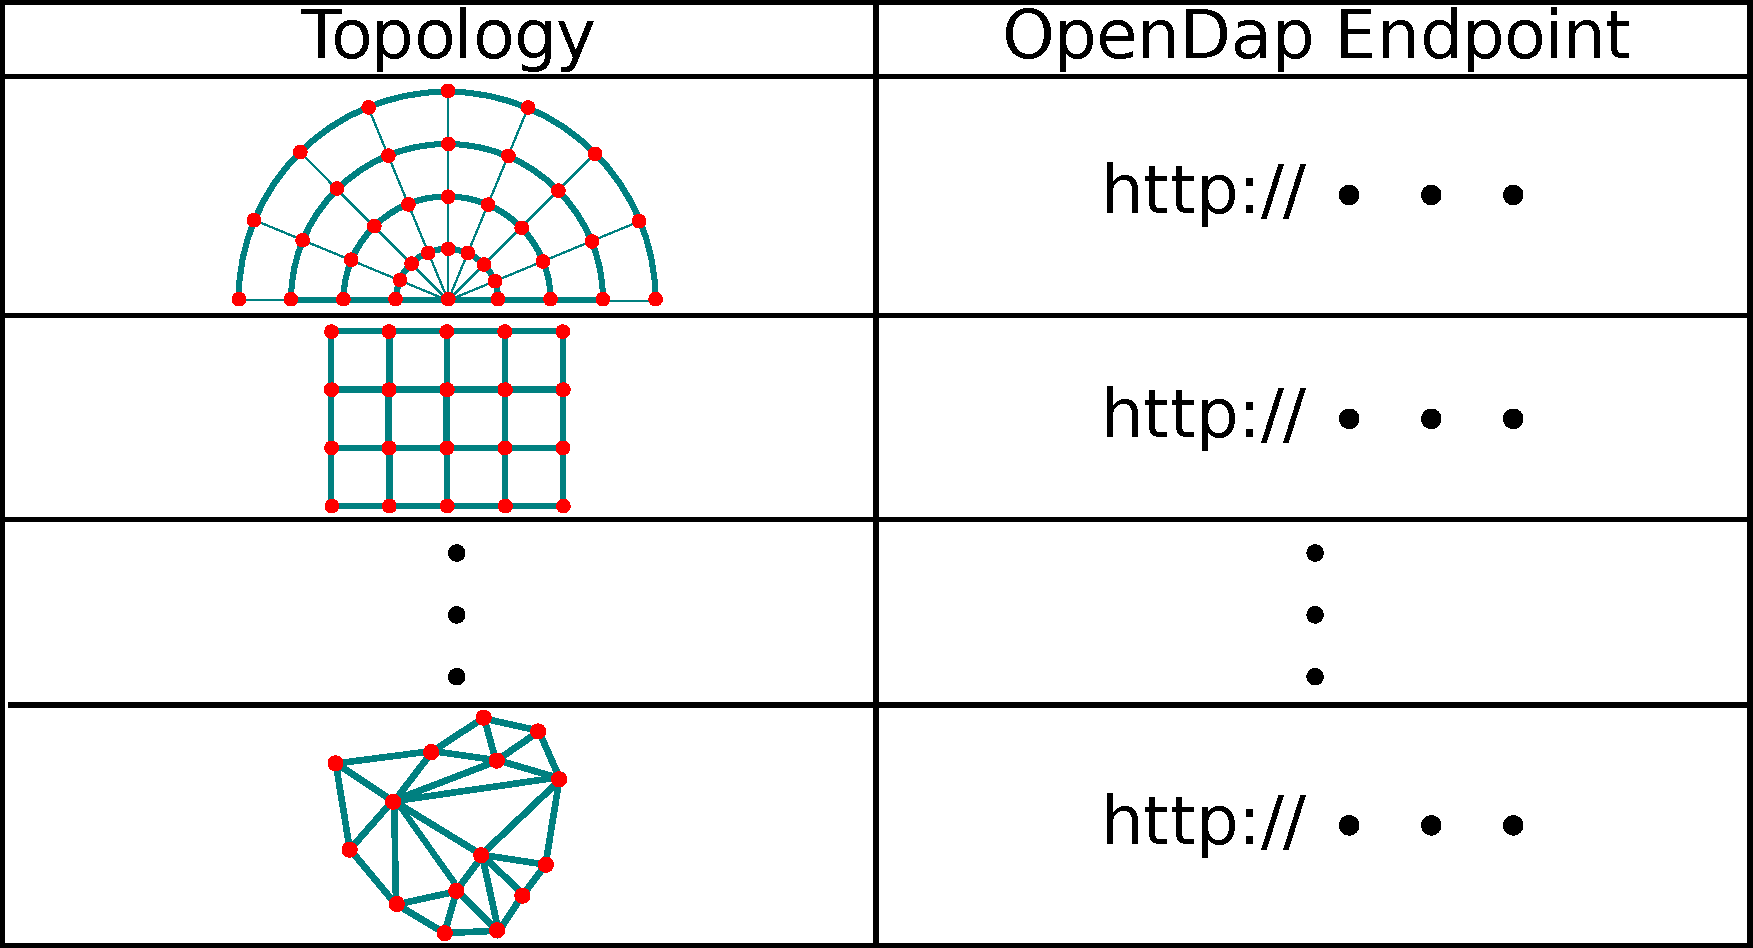
\includegraphics[width=0.6\columnwidth]{./figs/sciwms_db_topology_endpoints.pdf}
  \caption{\Sciwms{} topology and endpoint data store. Typologies are
    classified as \cgrid{} and \ugrid{} for efficient geospatial
    queries and remote model data access.}
  \label{fig:sciwms_topology_endpoints}
\end{figure}

\section{Deploying \sciwms{} for the U.S. \ioos{} \comt{} Testbed}
While \sciwms{} is a general software solution for geospatial
visualization, it is a key component in realizing the U.S. \ioos{}
\comt{} mission, facilitating qualitative model comparisons and
aggregation through a unified visualization
framework. Figure~\ref{fig:overview1} outlines the cyberinfrastructre
behind the deployment of \sciwms{} for the \comt{} project.

Raw coastal data is hosted by the Southeastern Universities Research
Association (\sura{}) on a dedicated server for the \comt{}
project~\cite{luettich12}. Each data set may consist of multiple files
in different formats, and may be the result of very different models
run by various institutions with disparate computing
resources. However, accompanying each dataset is an \ncml{} virtual
layer which exposes each dataset as a single \netcdf{} object which
may be accessed via
\opendap{}\footnote{http://www.opendap.org/}. Furthermore, the \ncml{}
facade presents a consistent set of meta information in accordance to
CF-Conventions~\cite{cf} so services like \sciwms{} can access the
data through a uniform interface.

The \noaa{}\footnote{National Oceanic and Atmospheric
  Administration}--\ngdc{}\footnote{National Geophysical Data Center}
Geoportal indexes public geophysical datasets and provides an \ogc{}
Catalogue Web Service (\csw{}) to query datasets by their metadata
attributes. Sci-wms queries the \ngdc{} Geoportal at regular intervals
updating both the topologies and \opendap{} links for all new or
modified datasets.

%% \sciwms{} is designed to be scalable and responsive to handle queries
%% for visualizations of any registered dataset by multiple users
%% simultaneously.

Currently, \Sciwms{} is used to visualize data from the first phase
groups of \ioos{} \comt{} program: {\em estuarine hypoxia, shelf hypoxia and
  coastal inundation}~\cite{luettich13}. For each modeling group,
\sciwms{} successfully generates visualizations from \adcirc{},
\fvcom{}, \selfe{} and \slosh{} models and serves as a use-case of how
\sciwms{} can be leveraged as a scalable solution for delivering
consistent visualizations of scientific data to a diverse community.

Figure~\ref{fig:adcirc_comp} shows a web-portal utilizing the
\sciwms{} backend to compare ADCIRC model output for Hurricane Ike
with water levels observed by NOAA Stations. Ongoing development is in
progress for \sciwms{} to support emerging geophysical datasets such
as ensemble model output as well as provide clear visual support for
the assessment and quantification of model skill and performance
metrics.
\begin{figure}[ht!]
  \centering
  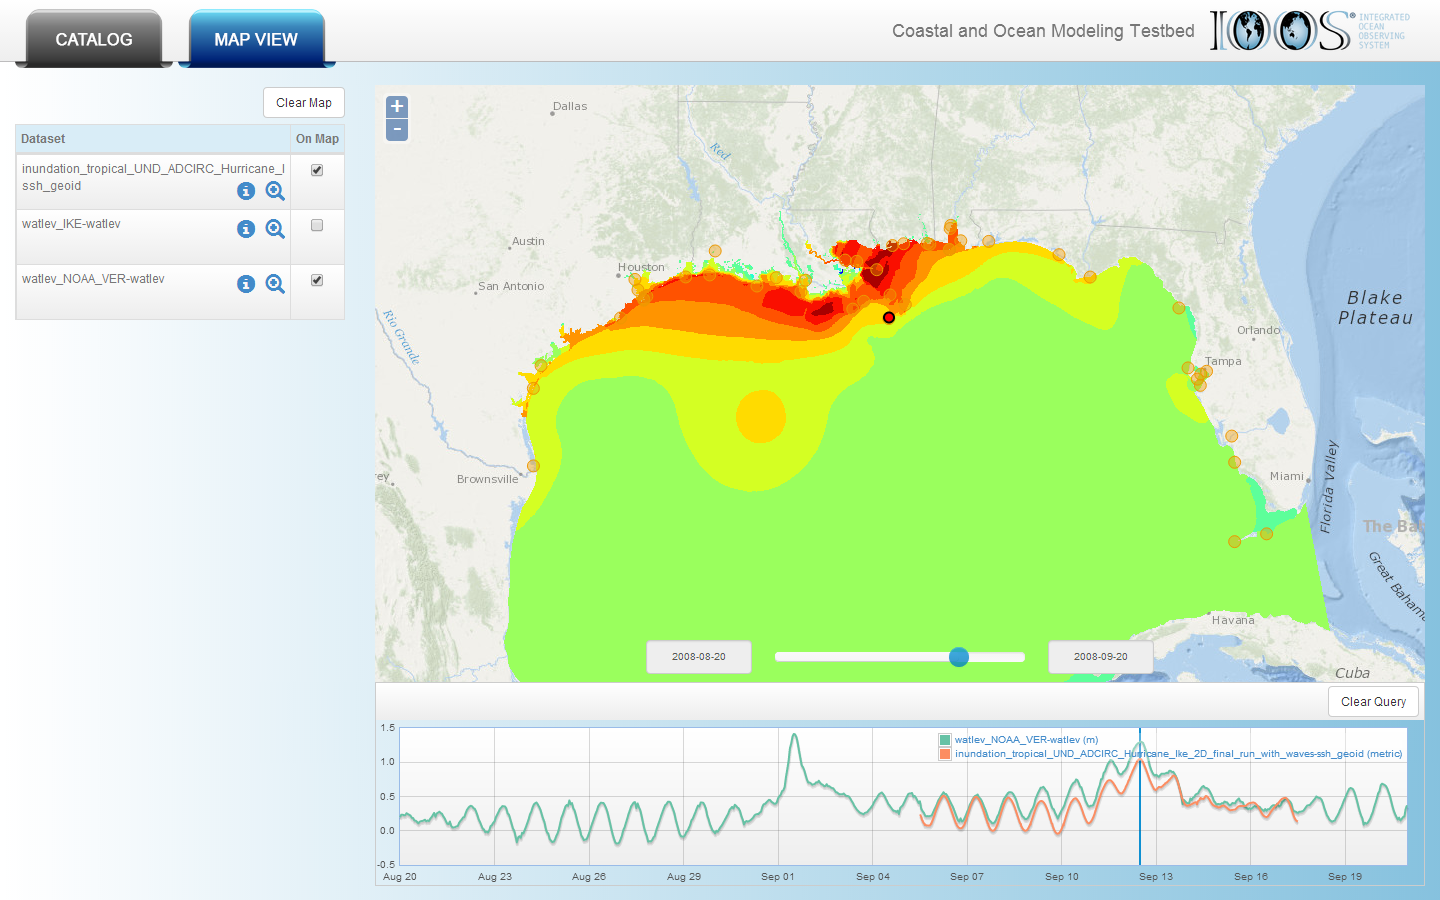
\includegraphics[width=0.9\columnwidth]{./figs/SciWMS_ModelObsComparison}
  \caption{Comparison of ADCIRC (unstructured topology) model results
    with observed water levels in the Norther Gulf of Mexico for
    Hurricane Ike. Verified observed water levels are from NOAA's
    Station 8760922 (red dot on map). The map shows modeled water
    levels (in meters above the geoid) at the peak of the storm in
    southern Louisiana. The time series plot shows both the modeled
    (green) and observed (orange) water levels. The vertical blue line
    in the time series plot corresponds to the current time of the
    map.}
  \label{fig:adcirc_comp}
\end{figure}
\bibliographystyle{ieeetr}
\bibliography{ci_mayer}
%% \bibliography{bibfile,benherzog}
\end{document}
